\documentclass[11pt,oneside]{book}


\usepackage[table]{xcolor}
\usepackage{titlesec}
\usepackage{mdframed}
\usepackage{wrapfig}

\colorlet{rulercolor}{gray!50}

\titleformat{\chapter}
  {\normalfont\sffamily\Large\fontfamily{phv}\selectfont}
  {\thechapter.}{.5em}{}
  [\vspace{.2ex}\color{rulercolor}\titlerule]
  
\newmdenv[leftmargin=20pt, rightmargin=20pt, 
skipabove=\topsep,skipbelow=\topsep,
backgroundcolor=gray!30,shadow=true,shadowsize=4,
roundcorner=10pt]{shadebox}

\newmdenv[leftmargin=30pt, rightmargin=30pt, 
skipabove=0pt,skipbelow=0pt,
backgroundcolor=gray!10]{mybox}

\usepackage{graphicx}
%%	using final option to force graphics to be included even in draft mode
%\usepackage[final]{graphicx}
\usepackage{paralist} % compact lists

%% Support sub-figures.
\usepackage{subfigure}

%% Make subsections numbered and included in ToC
\setcounter{secnumdepth}{3}
\setcounter{tocdepth}{2}

%% Make margins less ridiculous
\usepackage[margin=1.2in]{geometry}

%% Package to linebreak URLs in a sane manner.
\usepackage{url}

%% Define a new 'smallurl' style for the package that will use a smaller font.
\makeatletter
\def\url@smallurlstyle{%
  \@ifundefined{selectfont}{\def\UrlFont{\sf}}{\def\UrlFont{\small\ttfamily}}}
\makeatother
%% Now actually use the newly defined style.
\urlstyle{smallurl}
%% Make URLs clickable
\usepackage[colorlinks, bookmarks=true]{hyperref}
\usepackage[all]{hypcap}


%% Since I'm using the LaTeX Makefile that uses dvips, I need this
%% package to make URLs break nicely
\usepackage{breakurl}

\usepackage{array}

%% Make table cross pages.
\usepackage{longtable}
\usepackage[table]{xcolor}

%% Make links to captions point to the figure, not just the caption at bottom
\usepackage[all]{hypcap}

% create a shortcut to typeset table headings
\newcommand\tabhead[1]{\small\textbf{#1}}

\graphicspath{{figures/}} 
\DeclareGraphicsExtensions{.eps}

\setlength{\headheight}{15.2pt}

\usepackage{fancyhdr}
\pagestyle{fancy}
  \renewcommand{\chaptermark}[1]{\markboth{\MakeUppercase{\chaptername \ \thechapter \ \ #1}}{}}
  \fancyhf{}%clear all header and footer fields
    \fancyhead[LO]{\nouppercase{\rightmark}}
    \fancyhead[RE]{\nouppercase{\leftmark}}
       \fancyhead[RO,LE]{\thepage}
\def\chem#1#2{{{\scriptscriptstyle#1\atop\longrightarrow}\atop{\longleftarrow\atop\scriptscriptstyle#2}}}

\title{\textbf{Serious Game Stakeholder Experience Assessment Method (SGSEAM) \\
User Guide}}

\author{Yongwen Xu, Philip M. Johnson, Carleton A. Moore, Robert S. Brewer\\
\\
\em  Collaborative Software Development Laboratory \\
\em  Department of Information and Computer Sciences \\
\em  University of Hawai'i at Manoa\\
     \{yxu, johnson, cmoore, rbrewer\}@hawaii.edu}

\date{\today}

\begin{document}
  \maketitle
  \thispagestyle{empty}
  \tableofcontents
  \newpage
  
\chapter{SGSEAM Overview}
One of the benefits of using a serious game framework is that, if correctly designed, it will 
provide useful and reusable ``building blocks'' with which to develop a variety of serious 
games. Yet how are we to know if a serious game framework has been ``correctly designed''?

Serious Game Stakeholder Experience Assessment Method (SGSEAM) describes a method for 
assessing serious game frameworks from the stakeholder 
experience perspectives.  The goal of SGSEAM is to identify (a) major strengths of a serious game
framework, which aids the community by indicating features of the framework to emulate, and
(b) major shortcomings of the framework, which aids the community by indicating features to avoid.
The benefits of SGSEAM assessment are for the developers of serious game frameworks 
to learn and improve from the findings of the assessment.

SGSEAM is an assessment method instead of an evaluation method. The main purpose 
of an evaluation is to determine the quality of a program by formulating a judgment. An assessment, on 
the other hand, is nonjudgmental. SGSEAM does not try to judge a framework according to a 
standard, or to compare one framework against another. Instead, it is used to identify the major 
strengths and shortcomings of a framework to benefit  the developers of the framework.

\autoref{fig:overview} outlines the steps of the process of applying SGSEAM to a framework.

\begin{figure}[ht!]
  \center
  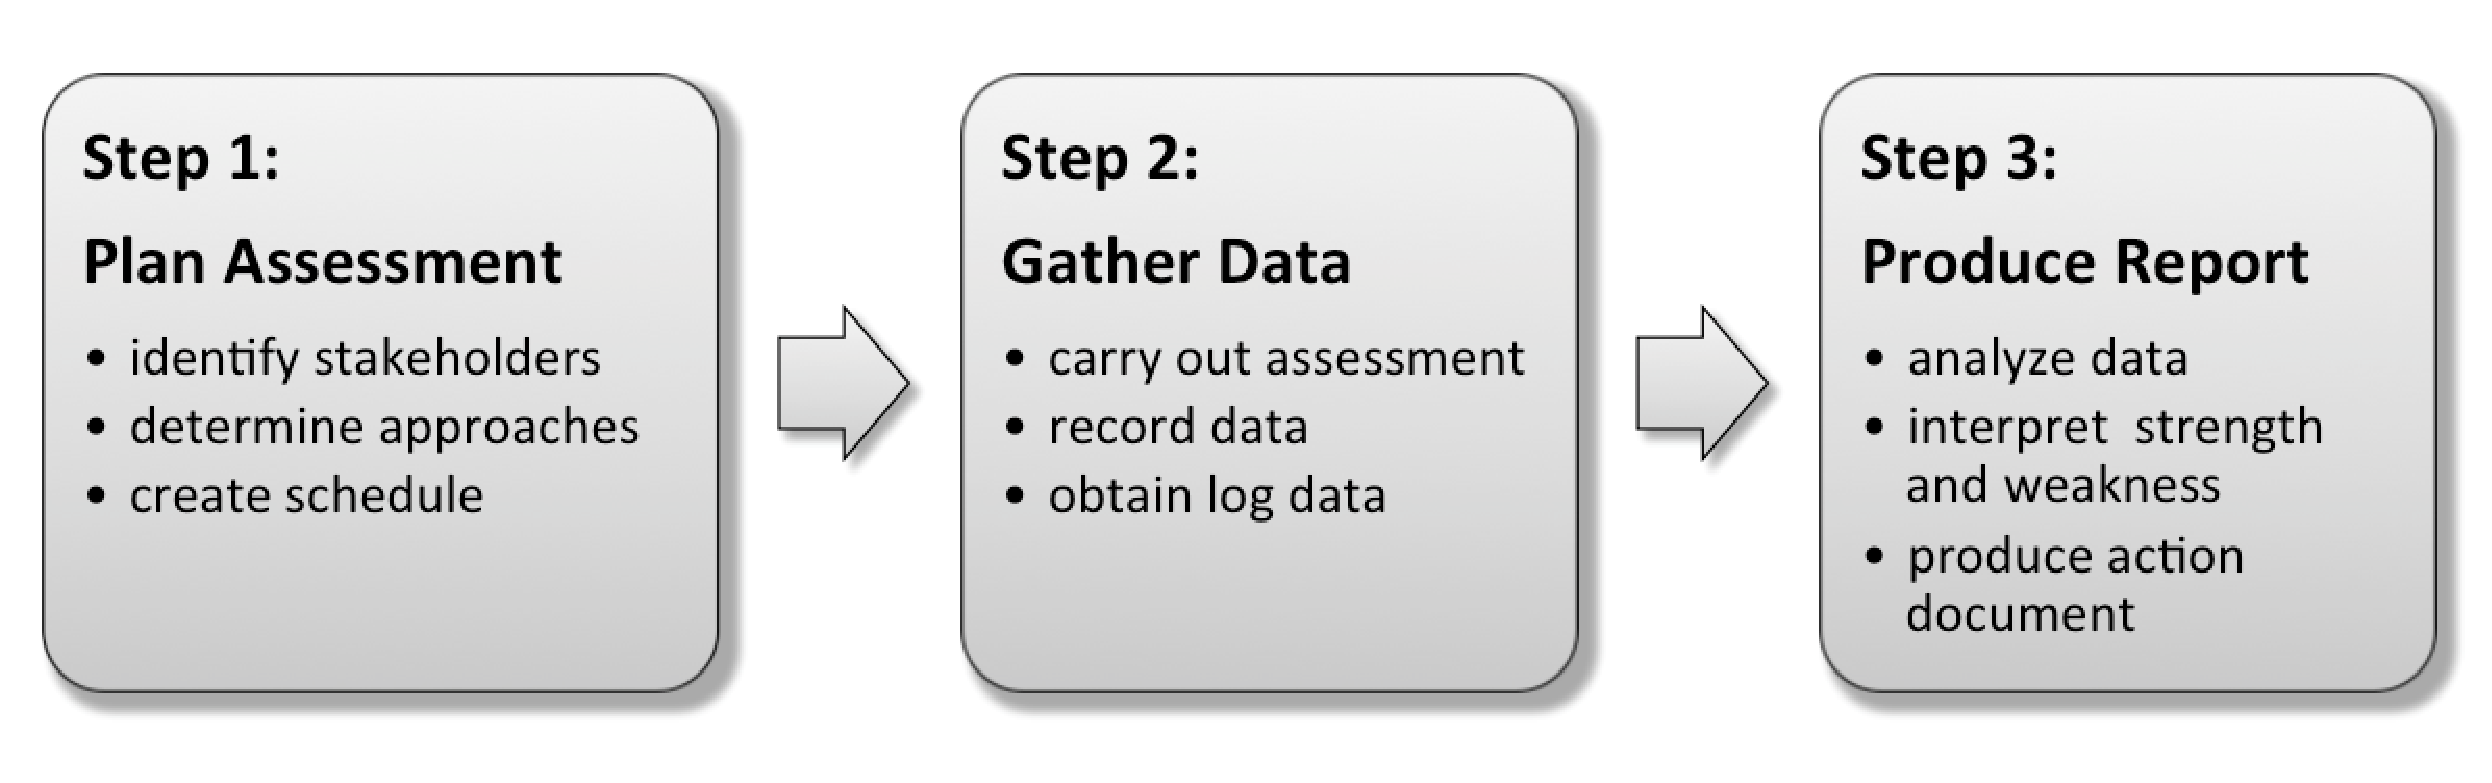
\includegraphics[width=0.8\columnwidth]{sgseam-steps}
  \caption{Applying SGSEAM to a framework}
  \label{fig:overview}
\end{figure}

There are three steps in the process of applying SGSEAM. Step one is to plan the assessment, including
 identifying the stakeholder and participants and creating the assessment plan. The deliverable for this 
 step is the assessment plan document. Step two is to gather data. The deliverable for this step is the 
 assessment data repository. Step three is to produce the strength and weakness report. The deliverable 
 for this step is the action document for framework improvement. The following chapters describe the 
 steps in details.

\chapter{Plan Assessment}

\section{Identify stakeholders}

\begin{shadebox}
\begin{wrapfigure}{l}{0.04\textwidth}
\vspace{-15pt}\hspace{-10pt}
    
\includegraphics[width=0.04\textwidth]{note-icon}
\end{wrapfigure}

Identify the stakeholders in each SGSEAM stakeholder class, write down their names and roles.

\end{shadebox}

SGSEAM assesses the experiences for the stakeholders listed in \autoref{table:stakeholders}. For each 
stakeholder, identify the population, the name and contact if possible. It is important to be able to contact 
the stakeholders in some way, either via email or phone, to get the feedback from their experiences with 
the framework.

\begin{table}[ht!]
  \centering
  \begin{tabular}{|p{0.2\columnwidth}|p{0.4\columnwidth}|p{0.3\columnwidth}|}
    \hline
    \tabhead{Stakeholder class} &
    \tabhead{Definition} &
    \tabhead{Examples} \\
    \hline
    Players &
    participate in the game produced by the framework. &
    students, residents \\
    \hline
    System admins &
    install and maintain the technological game infrastructure. &
    system admin, IT staffs \\
    \hline
    Game designer &
    design the content and game mechanics. &
    instructional designers, content experts \\
    \hline
    Game managers &
    manage the game during the period of game play.&
    sustainability coordinators, residential staffs\\
    \hline
    Game developers &
    develop customization, extend and enhance the game. &
    programmers, internal developers \\
    \hline
  \end{tabular}
  \caption{SGSEAM Stakeholders}
  \label{table:stakeholders}
\end{table}

\section{Determine assessment approach}

\begin{shadebox}
\begin{wrapfigure}{l}{0.04\textwidth}
\vspace{-15pt}\hspace{-10pt}
    
\includegraphics[width=0.04\textwidth]{note-icon}
\end{wrapfigure}
Determine the appropriate assessment approaches for each stakeholder.
\end{shadebox}

There are usually multiple assessment approaches for each stakeholder.  \autoref{table:approaches} provides 
an overview of the assessment method and the approaches. The appropriate assessment approaches should 
be determined according to the resource available. The approaches for a stakeholder is additive. The more 
approaches applied, the higher confidence of the assessment can be achieved. 

\begin{table}[ht!]
  \centering
  \begin{tabular}{|p{0.18\columnwidth}|p{0.28\columnwidth}|p{0.45\columnwidth}|}
    \hline
    \tabhead{Stakeholder}&
    \tabhead{Assessment Goal}&
    \tabhead{Assessment approaches} \\
    \hline
    Player&
    How does the framework affect and engage players?&
    	Pre-post effectiveness study(\ref{Pre-Post effectiveness study});\newline
	Self-reported usability metrics(\ref{Self-reported usability metrics});\newline
	Engagement metrics(\ref{Engagement metrics}) \\
    \hline
    System admin&
    How easy is it to install and maintain the system?&
    	Post-hoc system admin interview(\ref{Post-hoc system admin interview});\newline
	In-lab installation study(\ref{In-lab installation study}) \\
    \hline
    Game designer&
    How easy is it to design a game?&
    	Post-hoc designer interview(\ref{Post-hoc game designer interview});\newline
	In-lab game design study(\ref{In-lab game design study})\\
    \hline
    Game manager&
    How easy is it to manage a game?&
    	Post-hoc manager interview(\ref{Post-hoc game manager interview});\newline
	In-lab game management study(\ref{In-lab game management study})\\
    \hline
    Game developer&
    How easy is it to enhance the system?&
    	Post-hoc developer interview(\ref{Post-hoc game developer interview});\newline
	In-lab game development study(\ref{In-lab game development study}) \\
    \hline
  \end{tabular}
  \caption{SGSEAM approaches}
  \label{table:approaches}
\end{table}

The assessment approaches is categorized into in-vivo and in-vitro assessments. The in-vivo approaches, 
such as pre-post test, in-game surveys and post-hoc interviews, assess the real world instance of the game. 
The in-vitro approaches use in-lab experiments in a simulated environment. Different assessment
approaches will have different levels of rigor or validity. For example, the in-lab experiments (in-vitro) can 
enlist several subjects to perform the same pre-defined tasks and collect comparable data in a more 
controlled setting. It is rigor because of the generality achieved from the larger population of
participants under study. On the other hand, in-game surveys or interviews in the in-vivo approach typically 
collect data from different uncontroled settings with less rigor. But the in-invo data reflect the real world 
interaction between the stakeholders and the framework, thus provides better insights in the real world settings.

The following sections describe in detailed the different approaches for each stakeholder.  Each assessment 
approach describes the goal of the assessment, what data to collect, how to collect the data and how to 
analyze the data to obtain insights about the strengths and weaknesses of the framework from each 
stakeholder's perspective.

\subsection{Player assessment}

The goal of player assessment is to determine the effectiveness of the game
framework from player's perspective. It is essential that a game produced by a serious game
framework could achieve its intended "serious" purpose. The intended purposes of serious games are
always subject specific. For example, the desired effect of a serious game for
energy education and conservation is to increases players' energy literacy and
reduces their energy consumption during (and, hopefully, after) the game. A serious game for
language learning would have a very different desired effect. SGSEAM proposes three approaches for 
assessing the effectiveness from player's perspective.

\subsubsection{Player assessment approach: Pre-Post effectiveness study}
\label{Pre-Post effectiveness study}

This approach requires users of SGSEAM to first determine a set of domain-specific questions to assess the 
desired effects of their serious game. For example, a set of questionnaires on sustainability literacy, such as 
knowledge of power and energy, is used to assess the effectiveness of a serious game for sustainability education.

Once the domain-specific questionnaires are determined and designed, present this questionnaires as a 
survey to a random selection of the players before the game starts. After the game ends, present the same 
survey to the same players again. Compare the two set of survey response data to study if the game has an 
impact on the players regarding to the survey subjects. The extent of the changes reflected in the survey 
result indicates the degree of effectiveness of the serious game for this subject.

Serious games often engage players with resources of various types (energy, water, waste, etc.). Collect 
these measurements before, during, and after the game in order to acquire evidence regarding the potential 
impact upon player use of these resources.

\subsubsection{Player assessment approach: Self-reported usability metrics}
\label{Self-reported usability metrics}

This approach interviews players about their self-reported experiences with the game. Administrate the 
interview through online survey or face-to-face conversation, although we found that online survey is more 
cost effective than face-to-face conversation. If possible, implement the online survey as an activity inside the 
game. For example, the Makahiki serious game framework implements an online survey activity which 
incentivizes players to complete the survey by rewarding game points for the activity.

Use the usability questionnaires in \autoref{fig:usability-metrics} in the online survey or face-to-dace interview:\\

\begin{figure}[ht!]
\begin{mybox}
\begin{compactenum}
\item What did you like most about the game?
\item What did you found confusing?
\item What issues did you have while using the game?
\item What was the thing you liked the least about the game?
\item What can we do to improve the game?
\item It was easy to find what I was looking for on the website.  \\
	Strongly disagree  -  Disagree  -  Neutral  -  Agree  -  Strongly agree
\item The website was responsive. \\
	Strongly disagree  -  Disagree  -  Neutral  -  Agree  -  Strongly agree
\item The website provided adequate help in teaching me how to play. \\
	Strongly disagree  -  Disagree  -  Neutral  -  Agree  -  Strongly agree
\item I understood how to play. \\
	Strongly disagree  -  Disagree  -  Neutral  -  Agree  -  Strongly agree
\item this is something my friends should participate in. \\
	Strongly disagree  -  Disagree  -  Neutral  -  Agree  -  Strongly agree
\end{compactenum}
\end{mybox}
\caption{Player self-reported usability metrics questionnaires}
\label{fig:usability-metrics}  
\end{figure}

\subsubsection{Player assessment approach: Engagement metrics}
\label{Engagement metrics}

This approach calculates the engagement metrics to assess the extent of engagement from players and 
the impact of the game. The more engaging the game is, the more potential impact could be to the players.

Calculate as many as possible the player engagement metrics described in \autoref{figure:engagement-metrics} 
by analyzing the data from system log or other channels provided by the framework. The more metrics 
obtained, the better understanding of the extent of player engagement. 

\begin{figure}[ht!]
  \centering
  \rowcolors{1}{gray!10}{gray!10}
    \begin{tabular}{|p{0.2\columnwidth}|p{0.28\columnwidth}|p{0.32\columnwidth}|}
    \hline
    \tabhead{Metric} &
    \tabhead{Definition} &
    \tabhead{Mesure} \\
    \hline
    participation &
    percentage of players who play the game &
    the level of involvement from players \\
    \hline
    player &
    number of players per day &
    the frequency of players interact with the game \\
    \hline
    play time &
    play time of a player per day &
    the frequency of players interact with the game \\
    \hline
    submission &
    submissions of all player per day &
    the rate of players' completion of game activities \\
    \hline
    social interaction &
    social interaction of all player per day &
    the rate of in-game social interactions between players\\
    \hline
    game error &
    game errors per day &
    the rate of errors encountered by players during the game \\
    \hline
  \end{tabular}
  \caption{Player engagement metrics}
  \label{figure:engagement-metrics}
\end{figure}

With the exception of the game error metric, the higher value these metrics are, the higher engagement 
level the game has.

\subsection{System admin assessment}

System administrators are responsible for installing and maintaining the software infrastructure
for the game. Their tasks include the framework and dependency installation, maintain the database, 
backups, and so forth. The goal of system admin assessment is to determine to what extent the 
framework facilitates the system administration tasks from system admin's perspective. SGSEAM 
assesses how much time is required to install and maintain an instance of a serious game using the 
framework and the problems encountered  during the system admin process.
 
SGSEAM proposes two assessment approaches.

\subsubsection{System admin assessment approach: Post-hoc admin interview}
\label{Post-hoc system admin interview}

This approach assesses the system admin's experience using the post-hoc interview. The system admins 
are asked about their experience with the framework after they completed the installation and maintanence
 in the production system. The interview questions are described in \autoref{fig:system-admin-interview}.

\begin{figure}[ht!]
\begin{mybox}
\begin{compactenum}
\item How much time did you require to install the system and the dependencies?
\item What problems did you encounter when installing the system and the dependencies?
\item How much time did you require to maintain the system?
\item What problems did you encounter when maintaining the system?
\item Did you find it difficult to admin the system? What was difficult?
\end{compactenum}
\end{mybox}
\caption{System admin interview questionnaires}
\label{fig:system-admin-interview}  
\end{figure}

The interview should be tape-recorded. Once the interview is completed, qualitative data
analysis is performed against the interview data by doing: (1) transcribing the recordings; 
(2) coding (categorizing) the time and problems or difficulties encountered. These data reveal the 
strengths, weaknesses and the areas of improvement for the framework.

\subsubsection{System admin assessment approach: In-lab installation study}
\label{In-lab installation study}

This approach assesses the system admin's experience using the in-lab experimental study. First identify a group 
of participants who have some levels of system administration experience. Second, provide instructions on 
each installation steps, ask the participants to install the system according to the instructions, and ask them to record 
the time spent and problems encountered as they complete each step.

Once the experiment data is collected, categorize the reported problems and correlated with the reported time data 
to identify the areas of strength (less time spent) and weakness (more time spent and problems or difficulties). 

\subsection{Game designer assessment}

A game designer uses the serious game framework to design and create a serious game.
A serious game framework normally provides tools or interfaces for game designers
to facilitate the design of a game. For example, the framework provides interface to configure the game period, set up 
players, and tools to design individual game elements.

SGSEAM assesses the game designer stakeholder by addressing the following two questions: (a) How
much time is required to design an instance of a serious game using the framework? and (b) How
many, and how problematic are the errors that designers encounter during the design process?

There are two approaches for game designer assessment:

\subsubsection{Game designer assessment approach: Post-hoc designer interview}
\label{Post-hoc game designer interview}

This approach interviews the game designer(s) after they had completed the design of a serious game using the 
framework in a production system. The interview includes the questions described in \autoref{fig:game-designer-interview}.
 
\begin{figure}[ht!]
\begin{mybox}
\begin{compactenum}
\item How much time did you spend to complete each design task?
\item What problems did you encounter?
\item Did you find it difficult to configure? What was difficult?
\item Did you find it difficult to design a specific game? Which one, and what was difficult?
\end{compactenum}
\end{mybox}
\caption{Game designer interview questionnaires}
\label{fig:game-designer-interview}  
\end{figure}

The interview should be tape-recorded. After the interview, transcribed the recordings, code and categorize the reported 
time and problems to identify the strengths and weaknesses.

In addition, if possible, collect the system log data related to the game designing tasks, analyze the logs to find out the time 
spent and error encountered during the game designing tasks. Use the log data to verify the findings from the interview data.

\subsubsection{Game designer assessment approach: In-lab game design study}
\label{In-lab game design study}

This approach assesses the game designer experience using the in-lab experimental study.  First identify a group 
of participants who are somewhat familiar with the subject domain of the game. Second, provide instructions on 
each designing steps, ask the participants to design the game according to the instructions, ask them to record 
the time spent and problems encountered as they complete each step.

Once the experiment data is collected, categorize the reported problems and correlated with the reported time data 
to identify the areas of strength (less time spent) and weakness (more time spent and problems or difficulties). 

\subsection{Game manager assessment}

A game manager uses the serious game framework interface to manage the serious game that the game
designers created. It is possible that a game manager is also the game designer.
The examples of game management tasks includes managing player submissions, monitoring the game 
state, entering manual resource data, notifying winners of the game, etc.

SGSEAM assesses the game manager stakeholder with the following questions: (a) How much time is
required to manage an instance of a serious game using the framework? and (b) How many,
and how problematic are the errors that managers encounter during the design process?

SGSEAM proposes three approaches for assessment game manager's experience.

\subsubsection{Game manager assessment approach: Post-hoc manager interview}
\label{Post-hoc game manager interview}

This approach interviews the game manager(s) after they had managed a serious game using the framework 
in a production envrionment. The interview questions are described in \autoref{fig:game-manager-interview}.
 
\begin{figure}[ht!]
\begin{mybox}
\begin{compactenum}
\item How much time did you spend to complete each managing task?
\item What problems did you encounter?
\item Did you find it difficult to manage? What was difficult?
\end{compactenum}
\end{mybox}
\caption{Game manager interview questionnaires}
\label{fig:game-manager-interview}  
\end{figure}

The interview should be tape-recorded. After the interview, transcribed the recordings, code and categorize the reported 
time and problems to identify the strengths and weaknesses.

In addition, if possible, collect the system log data related to the game managing tasks, analyze the logs to find out the time 
spent and error encountered during the game managing tasks. Use the log data to verify the findings from the interview data.

\subsubsection{Game manager assessment approach: In-lab game management study}
\label{In-lab game management study}

This approach assess the game manager's experience using the in-lab game management study.  First identify a group 
of participants who are somewhat familiar with the subject domain of the game. Second, provide instructions on 
each managing tasks, ask the participants to complete the tasks following the instructions, ask them to record 
the time spent and problems encountered as they complete each task.

Once the experiment data is collected, categorize the reported problems and correlated with the reported time data 
to identify the areas of strength (less time spent) and weakness (more time spent and problems or difficulties). 

\subsection{Game developer assessment}

The game developer stakeholder is different from the game designer stakeholder, in that the
game designer stakeholder tailors the framework without requiring any software
development, while the game developer stakeholder enhances, corrects, and extends the system by
manipulating code. 

To investigate how easy it is to understand, extend, and debug a serious game
framework from a developer's perspective, SGSEAM assesses how much time it takes to develop an
enhancement to the game framework, and how many errors are encountered
during the process.

\subsubsection{Game developer assessment approach: Post-hoc developer interview}
\label{Post-hoc game developer interview}

This approach interviews the game developer(s) to assess their experiences of developing the game 
using the framework. The interview questions are described in \autoref{fig:game-developer-interview}.  
 
\begin{figure}[ht!]
\begin{mybox}
\begin{compactenum}
\item How much time did you spend developing a customization using the game framework?
\item What problem(s) did you encounter?
\item Did you find it difficult to understand, extend and debug the system? What was difficult?\\
\end{compactenum}
\end{mybox}
\caption{Game developer interview questionnaires}
\label{fig:game-developer-interview}  
\end{figure}

\subsubsection{Game developer assessment approach: In-lab game development study}
\label{In-lab game development study}

This approach assess the game developer's experience using the in-lab game development study.  
First identify the general development skills that the framework requires, such as the programming language. 
Second, identify a group of participants who have some levels of the required development skills. Third, provide 
requirement specification or instructions on how to develop a new enhancement to the system, ask the 
participants to complete the task, record the time spent and problems encountered as they works on the task.

Once the experiment data is collected, categorize the reported problems and correlated with the reported time data 
to identify the areas of strength (less time spent) and weakness (more time spent and problems or difficulties). 

\section {Choose participants}
\begin{shadebox}
\begin{wrapfigure}{l}{0.04\textwidth}
\vspace{-15pt}\hspace{-10pt}
    
\includegraphics[width=0.04\textwidth]{note-icon}
\end{wrapfigure}
Identify participants from each stakeholder class, Contact them and get consents for their participation.
\end{shadebox}

Once the assessment approaches are determined for each stakeholder class, the next step is to choose participants. 
Identify the  people from the each stakeholder class that may be willing to participate in the assessment, contact them 
and get consents for their participation. 

For example, in the case of pre-post effectiveness study approach for player assessment, this step randomly chooses a 
group of players and present a consent form before the online survey.  In the case of post-hoc game designer interview 
approach, the game designer of a real world game instance of the framework should be identified, contacted and consent 
for the participation in the assessment. When the in-lab game development experiment study is chosen, a group of game 
developers that meet the required development skills of the framework should be identified and contacted.

\section{Create assessment plan}
\begin{shadebox}
\begin{wrapfigure}{l}{0.04\textwidth}
\vspace{-15pt}\hspace{-10pt}
    
\includegraphics[width=0.04\textwidth]{note-icon}
\end{wrapfigure}
Create a schedule for each assessment, produce the assessment plan document.
\end{shadebox}

Once we decide what the assessment approaches and who the participants are, the next step is to create the assessment 
schedule and produce the assessment plan document. The document should include the detailed assessment plan for 
each stakeholder class. 

Depends on the assessment approach, the actual tasks of the assessment are different. The player pre-post 
effectiveness study requires the administration of online survey before and after the game. The game designer 
post-hoc interviews requires administration of interviews to the real world game designers of a production 
system. \autoref{figure:assessment-plan} shows an example of the assessment schedule broken down in the tasks 
in the plan document.

\begin{figure}[ht!]
  \centering
  \rowcolors{1}{gray!10}{gray!10}
  \begin{tabular}{|p{0.5\columnwidth}|p{0.15\columnwidth}|p{0.15\columnwidth}|}
    \hline
    \multicolumn{3}{|c|}{\tabhead{Game designer assessment approach: post-hoc interview}} \\
    \hline
    \tabhead{Task} &
    \tabhead{Estimated Start date} &
    \tabhead{Estimated End date} \\
    \hline
    Schedule the interview time & & \\
    \hline
    Administrate and record the interview & & \\
    \hline
    Obtain log data & & \\
    \hline
    Analyze the data & & \\
    \hline
    Interpret strength and weakness & & \\
    \hline
    Produce action document & & \\
    \hline
  \end{tabular}
  \caption{Assessment schedule in the plan document}
  \label{figure:assessment-plan}
\end{figure}


\chapter{Gather Data}
This step carries out the assessment, record the data, obtain log data, and refine the assessment plan if necessary. 
The output of this step is a data repository contains all the assessment data that can be analyzed in the next step.

\section{Carry out the assessment}
\begin{shadebox}
\begin{wrapfigure}{l}{0.04\textwidth}
\vspace{-15pt}\hspace{-10pt}
    
\includegraphics[width=0.04\textwidth]{note-icon}
\end{wrapfigure}
Carry out the assessment as described in the assessment plan.
\end{shadebox}

For each assessment approach, complete the tasks outlined in the assessment plan, gather the data when carrying out the 
assessment. In the case of game designer post-hoc interview approach, record the interview and take notes if necessary. 
Store all the data into a central data repository. 

\section{Obtain log data}
\begin{shadebox}
\begin{wrapfigure}{l}{0.04\textwidth}
\vspace{-15pt}\hspace{-10pt}
    
\includegraphics[width=0.04\textwidth]{note-icon}
\end{wrapfigure}
Obtain the log data from the framework, including all the interaction log from the each stakeholder.
\end{shadebox}

Talk to the technical staffs of the framework to find out what kind of log data is available. Obtain the log data in a format that 
is easy to analyze. For example, if the log data is in a database table, ask for the access to the table, or the CSV export of 
the table data. If the log data is in a log file, ask for the access to the file. Store the log data into the central data repository.

\chapter{Produce Strength and Weakness report}

This step analyzes all the data gathered from previous steps, interpret the strengths and weakness of the framework, 
and produce the action report regarding to what areas of the framework needs to improve on.

\section{Analyze data}
\begin{shadebox}
\begin{wrapfigure}{l}{0.04\textwidth}
\vspace{-15pt}\hspace{-10pt}
    
\includegraphics[width=0.04\textwidth]{note-icon}
\end{wrapfigure}
Analyze the data from the data repository.
\end{shadebox}
This step performs the data analysis from the data repository obtained from the previous step. For game designer assessment, 
perform queries from user interaction log data to find out the completion time for a certain user interaction task, for instance, the 
time for a game designer to complete the configuration of global game settings. For player assessment, calculate the 
engagement metrics from the game log. For post-hoc interview assessment approach, first transcribe the interview recording into 
text, code and categorize the responses from the interview questions. 
   
\section{Interpret strength and weakness}
\begin{shadebox}
\begin{wrapfigure}{l}{0.04\textwidth}
\vspace{-15pt}\hspace{-10pt}
    
\includegraphics[width=0.04\textwidth]{note-icon}
\end{wrapfigure}
Interpret strengths and weaknesses of framework from the data analysis.
\end{shadebox}


\section{Produce improvement action document}
\begin{shadebox}
\begin{wrapfigure}{l}{0.04\textwidth}
\vspace{-15pt}\hspace{-10pt}
    
\includegraphics[width=0.04\textwidth]{note-icon}
\end{wrapfigure}
Produce the action document for any improvement identified from the strength and weakness report.
\end{shadebox}

%% Use this for an alphabetically organized bibliography
%%\bibliography{sustainability,csdl-trs,gamification,yxu}
%%\bibliographystyle{plain}

\end{document}